%% uctest.tex 11/3/94
%% Copyright (C) 1988-2004 Daniel Gildea, BBF, Ethan Munson.
%
% This work may be distributed and/or modified under the
% conditions of the LaTeX Project Public License, either version 1.3
% of this license or (at your option) any later version.
% The latest version of this license is in
%   http://www.latex-project.org/lppl.txt
% and version 1.3 or later is part of all distributions of LaTeX
% version 2003/12/01 or later.
%
% This work has the LPPL maintenance status "maintained".
% 
% The Current Maintainer of this work is Daniel Gildea.

\documentclass[12pt]{ucthesis}
\def\dsp{\def\baselinestretch{2.0}\large\normalsize}
\dsp

%%BIBLIOGRAPHY- This uses biber/biblatex to generate bibliographies according to the
%%Unified Style Sheet for Linguistics
\usepackage[main=american, german]{babel}% Recommended
\usepackage{csquotes}% Recommended
\usepackage[backend=biber,
        style=unified,
        maxcitenames=3,
        maxbibnames=99,
        natbib,
        url=false]{biblatex}
\addbibresource{Dissertation.bib}
\setcounter{biburlnumpenalty}{100}  % allow URL breaks at numbers
% \setcounter{biburlucpenalty}{100}   % allow URL breaks at uppercase letters
% \setcounter{biburllcpenalty}{100}   % allow URL breaks at lowercase letters

%%TYPOLOGY  
\usepackage{tipa} %International Phonetic Alphabet
\usepackage[colorlinks,allcolors={black},urlcolor={blue}]{hyperref} %allows for hyperlinks and pdf bookmarks 
\usepackage{graphicx}	%Inserting graphics, pictures, images 		
\usepackage{fontspec} %Selection of fonts must be ran in XeLaTeX or LuaLateX
\usepackage{amssymb} %Math symbols
\usepackage{amsmath} % Mathematical enhancements for LaTeX
\usepackage{multicol} %Multicolumn text
\usepackage{enumitem} %Allows for continuous numbering of lists over examples, etc.
\usepackage{multirow} %Useful for combining cells in tablesbrew 
\usepackage{booktabs} %Enhanced tables
\usepackage{underscore} %Allows for underscores in text mode
% \usepackage[colorlinks,allcolors={black},urlcolor={blue}]{hyperref} %allows for hyperlinks and pdf bookmarks
% \usepackage{url} %allows for urls
% \def\UrlBreaks{\do\/\do-} %allows for urls to be broken up
% \usepackage[normalem]{ulem} %strike out text. Handy for syntax
\usepackage{tcolorbox}
% \usepackage{todonotes} % Creates todo marginalia

%%FONTS
\setmainfont{Libertinus Serif}
\setsansfont{Libertinus Sans}
% \setmonofont[Scale=MatchLowercase]{Libertinus Mono}

%%PACKAGES FOR LINGUISTICS
%\usepackage{OTtablx} %Generating tableaux with using TIPA
% \usepackage[noipa]{OTtablx} % Use this one generating tableaux without using TIPA
%\usepackage[notipa]{ot-tableau} % Another tableau drawing packing use for posters.
% \usepackage{linguex} % Linguistic examples
% \usepackage{langsci-linguex} % Linguistic examples
\usepackage{langsci-gb4e} % Language Science Press' modification of gb4e
% \usepackage{langsci-avm} % Language Science Press' AVM package
\usepackage{tikz} % Drawing Hasse diagrams
\usetikzlibrary{decorations.pathreplacing}
% \usepackage{pst-asr} % Drawing autosegmental features
% \usepackage{pstricks} % required for pst-asr, OTtablx, pst-jtree.
% \usepackage{pst-jtree} 	% Syntax tree draawing software
% \usepackage{tikz-qtree}	% Another syntax tree drawing software. Uses bracket notation.
% \usepackage[linguistics]{forest}	% Another syntax tree drawing software. Uses bracket notation.
% \usepackage{ling-macros} % Various linguistic macros. Does not work with linguex.
% \usepackage{covington} % Another linguistic examples package.
\usepackage{leipzig} %	Offers support for Leipzig Glossing Rules

%%LEIPZIG GLOSSING FOR ZAPOTEC
\newleipzig{el}{el}{elder} % Elder pronouns
\newleipzig{hu}{hu}{human} % Human pronouns
\newleipzig{an}{an}{animate} % Animate pronouns
\newleipzig{in}{in}{inanimate} % Inanimate pronouns
\newleipzig{pot}{pot}{potential} % Potential Aspect
\newleipzig{cont}{cont}{continuative} % Continuative Aspect
\newleipzig{stat}{stat}{stative} % Stative Aspect
\newleipzig{and}{and}{andative} % Andative Aspect
\newleipzig{ven}{ven}{venative} % Venative Aspect
% \newleipzig{res}{res}{restitutive} % Restitutive Aspect
\newleipzig{rep}{rep}{repetitive} % Repetitive Aspect

%%MACROS
\newcommand{\sub}[1]{\textsubscript{#1}}
\newcommand{\supr}[1]{\textsuperscript{#1}}
\providecommand{\lsptoprule}{\midrule\toprule}
\providecommand{\lspbottomrule}{\bottomrule\midrule}
\newcommand{\fittable}[1]{\resizebox{\textwidth}{!}{#1}}

\begin{document}

% Declarations for Front Matter

\title{Voice Quality and Tone at the Phonetics-Phonology Interface}
\author{Mykel Loren Brinkerhoff}
\degreeyear{2025}
\degreemonth{June}
\degree{DOCTOR OF PHILOSOPHY}
\chair{Professor Grant McGuire}
\committeememberone{Professor Jaye Padgett}
\committeemembertwo{Professor Ryan Bennett}
\committeememberthree{Professor Marc Garellek}
\numberofmembers{4} %% (including chair) possible: 3, 4, 5, 6
\deanlineone{Peter Biehl}
\deanlinetwo{Vice Provost and Dean of Graduate Studies}
\deanlinethree{}
\field{Linguistics}
\campus{Santa Cruz}

\begin{frontmatter}

\maketitle
\copyrightpage

\tableofcontents
\listoffigures
\listoftables

\begin{abstract}
Theses have elements.  Isn't that nice?

\end{abstract}
\begin{dedication}
\null\vfil
{\large
\begin{center}
To myself,\\\vspace{12pt}
Mykel Loren Brinkerhoff,\\\vspace{12pt}
the only person worthy of my company.
\end{center}}
\vfil\null
\end{dedication}
\begin{acknowledgements}
    When it comes to acknowledgements, there are so many words that could be said, but they often feel awkward and do not actually . There are many people who have helped me along the way, from my family to my friends, to my colleagues and mentors. I am grateful to all of them. 

    % I would like to thank my advisor, Professor Grant McGuire, for his guidance and support throughout my time in graduate school. I would also like to thank my committee members, Professor Jaye Padgett, Professor Ryan Bennett, and Professor Marc Garellek, for their feedback and advice.

    % I would like to thank my family for their love and support. I would also like to thank my friends for their encouragement and understanding.

    % Finally, I would like to thank my wife, Betsy for their patience and understanding. I could not have done this without them.
\end{acknowledgements}



\end{frontmatter}

%--------------------------------------------------------------------------
%  Introduction
%--------------------------------------------------------------------------

%--------------------------------------------------------------------------
\chapter{Introduction} \label{chap:introduction}
%--------------------------------------------------------------------------


%--------------------------------------------------------------------------
\section{What is Voice Quality} \label{sec:voice_quality}
%--------------------------------------------------------------------------
Voice quality describes the state of the larynx during phonation, when the vocal folds are set in motion. Languages make use of voice quality for paralinguistic purposes, such as conveying indexation of ``biological, psychological, and social characteristics of the speaker'' \citep{laverVoiceQualityIndexical1968} and racial identity \citep{podesvaStanceWindowLanguageRace2016}. 

Voice quality is also used linguistically. In English, it is often the case that we use creaky voice to indicate that we are at the end of an utterance \citep[e.g.,][]{garellekProductionPerceptionGlottal2013}. In many other languages, voice quality is used as part of the phonological system. Most famously, Gujarati has a phonemic contrast between breathy and modal voice in vowels \citep[e.g.,][]{fischer-jorgensenPhoneticAnalysisBreathy1968,espositoContrastiveBreathinessConsonants2012, khanPhoneticsContrastivePhonation2012,espositoDistinguishingBreathyConsonants2019}. 

\citet{espositoCrossLinguisticPatterns2020}

%--------------------------------------------------------------------------
\section{Voice Quality and Tone} \label{sec:voice_quality_and_tone}
%--------------------------------------------------------------------------

%--------------------------------------------------------------------------
\section{Voice Quality and Phonation} \label{sec:voice_quality_and_phonation}
%--------------------------------------------------------------------------

% In other languages, voice quality can be used to distinguish between phonemes, such as in Jalapa Mazatec, where voice quality is used to distinguish between voiced and voiceless stops \citep{merrillVoiceQualityJalapa2011}. Voice quality is also used to convey information about the speaker's emotional state, such as in the case of breathiness, which is often associated with sadness \citep{hentonBreathinessVoiceQuality1996}.

%--------------------------------------------------------------------
%
% File: 2.SLZ.tex
% Author: Mykel Loren Brinkerhoff
% Description: Chapter on the Vowels and suprasegmentals in Santiago Laxopa Zapotec
%
%--------------------------------------------------------------------




\chapter{Vowels and suprasegmentals in Santiago Laxopa Zapotec} \label{ch:SLZ}

%-------------------------
\section{Introduction} \label{sec:SLZ-intro}
%-------------------------

Santiago Laxopa Zapotec (SLZ; \textit{Dilla'xhunh Laxup} [diʒaˀʐun lːaʂupʰ]) is a Northern Zapotec language spoken by approximately 1000 people in the municipality of Santiago Laxopa, Ixtlán,Oaxaca, Mexico and in diaspora communities throughout Mexico and the United States \citep{adlerAcousticsPhonationTypes2016,adlerDerivationVerbInitiality2018,foleyForbiddenCliticClusters2018,foleyExtendingPersonCaseConstraint2020}. 
According to \citet{smith-starkAlgunasIsoglosasZapotecas2007}, SLZ is part of the macro variety of Cajonos Zapotec, which also includes Zoogocho Zapotec, Yatzachi Zapotec, Yalálag Zapotec, Tabaá Zapotec, Lachirioag Zapotec, and several other varieties spoken in the Sierra Norte of Oaxaca, Mexico.

\begin{figure}[!h]
    \centering
    \includegraphics[width=0.9\textwidth]{images/SantiagoLaxopa.jpeg}
    \caption{Santiago Laxopa taken by Beto Diaz, a resident of Santiago Laxopa.}
    \label{fig:SantiagoLaxopa}
\end{figure}



%-------------------------
\section{Vowels in Santiago Laxopa Zapotec} \label{sec:SLZ-vowels}
%-------------------------

SLZ exhibits a four-vowel inventory; see Table~\ref{tab:SLZ_vowel_chart}. This type of vowel inventory is very common among Sierra Norte Zapotecs. Most varieties have the vowels /i/, /e/, /a/, and /o/ \citep{nellisFortisLenisCajonos1980,jaegerInitialConsonantClusters1982,butlerh.DiccionarioZapotecoYatzachi1997,avelinobecerraTopicsYalalagZapotec2004,longDiccionarioZapotecoSan2005,sonnenscheinDescriptiveGrammarSan2005}. 

\begin{table}[!h]
    \centering
    \caption{Vowel qualities in Santiago Laxopa Zapotec.}
    \label{tab:SLZ_vowel_chart}
    \begin{tabular}{lccc}
        \lsptoprule
        &  front& central  & back \\
        \midrule
        high   	&  i  &     &   u$\thicksim$o \\
        mid    	&  e  &   	& 	\\
        low   	&     &  a 	&	  \\
        \lspbottomrule
    \end{tabular}
\end{table}

The vowel /o/ is marginal in SLZ's lexicon, only appearing in a few lexical items such as the diminutive classifier \textit{do'}. Instead, this vowel is replaced by /u/ in most cases. However, this difference is not universal among all speakers in the community. For the most part older speakers exhibit the vowel /o/ in their speech, while younger speakers tend to replace it with /u/. Most speakers, when asked, classify the two back rounded vowels as the same phoneme and view them as a dialectal feature between the different pueblos. For example, in neighboring San Bartolomé Zoogocho the /u/ vowel is very marginal and has led \citet{sonnenscheinDescriptiveGrammarSan2005} to describe the language as having only four vowels.It is interesting to note that everywhere that SLZ has the vowels /u/ or /o/, Zoogocho only has /o/. Further evidence for this comes from plotting the vowels along the first two formants. As shown in Figure~\ref{fig:SLZvowels}, the vowels /o/ and /u/ occupy nearly identical vowel spaces.

\begin{figure}[!h]
    \centering
    \includegraphics[width = 0.9\linewidth]{images/slz_vowels.eps}
    \caption{Vowel space of Santiago Laxopa Zapotec. The ellipses around each vowel mean represents 1 standard. The scale of the axes are in barks with their corresponding Hz values.}
    \label{fig:SLZvowels}
\end{figure}

Additional evidence for the overlap of /o/ and /u/ can be measured with a combination of Pillai scores \citep{pillaiNewTestCriteria1955,hayFactorsInfluencingSpeech2006,nyczBestPracticesMeasuring2014} and Bhattarcharyya's Affinity \citep{bhattacharyyaMeasureDivergenceTwo1943,johnsonQuantifyingOverlapBhattacharyyas2015,warrenQualityQuantityNew2018,strellufChapter3Low2018}. Both of these measures show what degree of overlap exists between two different items in some space. Their use in linguistics has been used mainly to show the process of complete and partial mergers between vowels, such as the \textsc{near-square} vowel merger in New Zealand English \citep{hayFactorsInfluencingSpeech2006}. The Pillai scores and Bhattacharyya's Affinity show that the vowels /o/ and /u/ are nearly identical in their vowel space; see Table~\ref{tab:SLZvowels_affinity}.

\begin{table}[!h]
    \centering
    \caption{Pillai scores and Bhattacharyya's Affinity for /o/ and /u/ in SLZ.}
    \label{tab:SLZvowels_affinity}
    \begin{tabular}{lcc}
        \lsptoprule
        &  Pillai score & Bhattacharyya's Affinity \\
        \midrule
        All speakers & 0.157 & 0.892 \\
        Females & 0.138 & 0.890 \\
        Males   & 0.224 & 0.858 \\
        \lspbottomrule
    \end{tabular}
\end{table}

In interpreting these results, Pillai scores range from 0 to 1, with 0 indicating overlap and 1 indicating complete no overlap. Bhattacharyya's Affinity ranges from 0 to 1, with 0 indicating no overlap and 1 indicating complete overlap. The results show that the overlap between /o/ and /u/ is not complete, but it is also not completely separating. This is consistent with the observations made by myself and other researchers for this variety (Toosarvandani, p.c.). 

In summary, we can conclude that SLZ is similar to other Northern Zapotec varieties in having a four-vowel inventory. The vowel /o/ is marginal in the lexicon and is often replaced by /u/ in younger speakers. The vowels /o/ and /u/ occupy nearly identical vowel spaces, and the overlap between the two vowels is not complete but is also not completely separating. 

%-------------------------
\section{Voice Quality contrasts in Santiago Laxopa Zapotec} \label{sec:SLZ-voicequality}
%-------------------------
Most Zapotec languages also make use of contrastive voice qualities (see \cite{ariza-garciaPhonationTypesTones2018} for an overview and typology of the voice quality contrasts in the Zapotec language family), with SLZ being no exception. SLZ
has a four-way voice quality contrast: modal, breathy, checked, and rearticulated. These contrasts are exemplified in the minimal quadruple in (\ref{ex:SLZphonation}).

\ea \label{ex:SLZphonation} Four-way near minimal phonation contrast
    \ea \textit{yag}  /çag\supr{L}/ `tree; wood; almúd (unit of measurement approximately 4kg)'
    \ex \textit{yah}  /ça̤\supr{L}/ `metal; rifle; bell'
    \ex \textit{yu'}  /çuˀ\supr{L}/  `cooking pot'
    \ex \textit{ya'a}  /çaˀa\supr{L}/  `market'
    \z
\z
SLZ shares with most Zpaotec varities, two types of creaky voice: checked and rearticulated. Checked vowels are characterized by an abrupt glottal closure which cuts the vowel short. This phonation is sometimes realized as a period of creakiness at the end of the vowel.

Among speakers of SLZ, there is a large amount of inter- and intra-speaker variability in how the rearticulated vowels are produced. Some speakers produce these vowels with a full glottal stop in the middle of the vowel, others produce a vowel with apparent modal voice but with a drop in amplitude (similar to what \cite{gerfenProductionPerceptionLaryngealized2005} found for some Mixtec varities), while others produce creaky voice throughout the entire vowel. Some speakers produce a combination of these unique productions. Overall, these rearticulated vowels are proiduced with some form of manipulation of glottal closure or apmlitude drop in the middle of the vowel.

[INSERT SPECTROGRAMS OF CHECKED AND REARTICULATED VOWELS]

SLZ is also unique in regards to its voice quality contrasts because it is a Northern Core Zapotec that has developed breathy voice, which has not been described in any of the neighboring Sierra Norte varieties \citep{nellisFortisLenisCajonos1980,jaegerInitialConsonantClusters1982,butlerh.DiccionarioZapotecoYatzachi1997,avelinobecerraTopicsYalalagZapotec2004,sonnenscheinDescriptiveGrammarSan2005,longDiccionarioZapotecoSan2005}.\footnote{Breathy voice in Zapotec languages, however, is common in Central Valley Zapotecs \citep{munroDiCsyonaaryTee1999,espositoSantaAnaValle2004,espositoVariationContrastivePhonation2010,uchiharaToneRegistrogenesisQuiavini2016,ariza-garciaPhonationTypesTones2018}.} Breathy voice is characterized by a raspiness throughout the whole vowel or a portion of the vowel depending on the speaker.

[INSERT SPECTROGRAM OF BREATHY VOWEL]


%-------------------------
\section{Tonal contrasts in Santiago Laxopa Zapotec} \label{sec:SLZ-tones}
%-------------------------
One of the most well known features of all Oto-Manguean languages is the fact that they are tonal languages and exhibit a large range of tonal systems \citep{pikeProblemsZapotecTone1948,renschComparativeOtomangueanPhonology1976,josserandMixtecDialectHistory1983,silvermanLaryngealComplexityOtomanguean1997,beamdeazconaProblemsZapotecTone2007,dicanioItunyosoTrique2010,dicanioCoarticulationToneGlottal2012,elliottChicahuaxtlaTriqui2016,
campbellOtomangueanHistoricalLinguistics2017a,campbellOtomangueanHistoricalLinguistics2017b,
lillehaugenOtomangueanLanguages2019,eischensTonePhonationPhonologyPhonetics2022}. SLZ has a five-way tonal contrast which consists of three level tones (high, mid, low) and two contour tones (rising and falling). 

\citet{brinkerhoffTonalPatternsTheir2022}

%------------------------------------
\section{Interactions between tone and voice quality} \label{sec:SLZ-interaction}
%------------------------------------

% Santiago Laxopa Zapotec (SLZ; \textit{Dilla'xhunh Laxup} [diʒaˀʐun laʂup]) is a Northern Zapotec language spoken by approximately 1000 people in the municipality of Santiago Laxopa, Ixtlán District in the Sierra Norte of Oaxaca, Mexico \citep{adlerAcousticsPhonationTypes2016,adlerDerivationVerbInitiality2018,foleyForbiddenCliticClusters2018,foleyExtendingPersonCaseConstraint2020}.\footnote{This macro variety is also sometimes called Cajonos Zapotec and comprises the dialects of Zoogocho Zapotec, Yatzachi Zapotec, Yalálag Zapotec, Tabaá Zapotec, and Lachirioag Zapotec \citep{smith-starkAlgunasIsoglosasZapotecas2003}.} It is mutually intelligible with San Bartolomé Zoogocho Zapotec \citep{longDiccionarioZapotecoSan2005,sonnenscheinDescriptiveGrammarSan2005}. SLZ has a fairly standard five-vowel inventory; see Table~\ref{tab:SLZvowels}.\footnote{The /o/ vowel is marginal in the lexicon for SLZ and only appears in a few lexical items. In neighboring San Bartolomé Zoogocho the /u/ vowel is very marginal and has led \citet{sonnenscheinDescriptiveGrammarSan2005} to describe the language as having only four vowels. It is interesting to note that everywhere that SLZ has the vowels /u/ or /o/, Zoogocho only has /o/. When plotting the vowel spaces and looking for outliers in the data based on F1 and F2, I noticed that the vowels /o/ and /u/ occupy nearly identical vowel spaces.}


		
% Among Zapotecan languages, it is quite common for languages to make use of contrastive phonation \citep[e.g.,][]{avelinobecerraTopicsYalalagZapotec2004,longDiccionarioZapotecoSan2005,avelinoAcousticElectroglottographicAnalyses2010,lopeznicolasEstudiosFonologiaGramatica2016,chavez-peonInteractionMetricalStructure2010}. In \posscitet{ariza-garciaPhonationTypesTones2018} typological description of phonation in Zapotecan languages, most have two to three phonation types which are described as involving creaky phonation or a glottal closure that is considered a vocalic feature. \citet{ariza-garciaPhonationTypesTones2018} additionally notes that breathy phonation is quite rare among Zapotecan languages, with only three languages in her typological study having this phonation type. Based on this typological data, she claims that breathy phonation is a recent innovation and is restricted to the Valley Zapotec languages only. However, SLZ, as a Northern Zapotec language, presents evidence to the contrary. SLZ has a four-way phonation contrast: modal, breathy, checked, and laryngealized. These contrasts are exemplified in the minimal quadruple in (\ref{ex:YA}).
% \ea \label{ex:YA} Four-way near minimal phonation contrast
%     \ea \textit{yag}  /çag\supr{L}/ `tree; wood; almúd (unit of measurement approximately 4kg)'
%     \ex \textit{yah}  /ça̤\supr{L}/ `metal; rifle; bell'
%     \ex \textit{yu'}  /çuˀ\supr{L}/  `earth'
%     \ex \textit{ya'a}  /çaˀa\supr{L}/  `market'
%     \z 
% \z 

% In representing the checked and laryngealized vowels, I follow the same procedure as other authors (e.g., \citet{avelinoAcousticElectroglottographicAnalyses2010, uchiharaToneRegistrogenesisQuiavini2016}) in representing the ``glottal stop'' element as a superscript glottal stop in the IPA transcription (i.e., [aˀ] or [aˀa]). This is primarily done as a way of standardizing the variable pronunciation of the glottal element in Zapotec, ranging from a full glottal stop (i.e., [aʔ] or [aʔa]) to a creaky portion of the vowel (i.e., [aa̰] or [aa̰a ]).  
% Theoretically, one could argue that checked and laryngealized vowels are not actually phonation types but involve a glottal stop consonant, either as a syllabic onset or coda. It is indeed logical that this could be the case. However, much work has shown that this cannot be true in Zapotec for the laryngealized vowels, which have a glottal closure in their center. \citet{chavez-peonInteractionMetricalStructure2010} summarizes this work and offers six reasons why these ``glottal stops" are a vocalic feature, not a consonant in laryngealized vowels. The first reason has to do with the distribution of the glottal stop. If it is indeed a coda or onset, then we would expect it could also occur word-initially or in consonant clusters. This does not happen in SLZ or other Zapotec languages \citep{jaegerInitialConsonantClusters1982}. Another point that he raises is that when linguists ask native language consultants about how many syllables or beats the word has, they treat laryngealized vowels as if they only had a single beat.\footnote{This is something Maya Wax Cavallaro and I tested with one of our consultants. The only times that they said one of these laryngealized vowels was not a single beat was when they had differing vowel qualities on either side of the glottal closure (e.g., \textit{bi'a} [biˀa] `fly (insect)').} These and other points raised by \citeauthor{chavez-peonInteractionMetricalStructure2010} are presented in (2). 

% \ea  Summary: glottal stop as a vocalic feature in laryngealized vowels (adapted from \cite{chavez-peonInteractionMetricalStructure2010}).
%     \ea /ʔ/ defective distribution (not in onset, not in clusters)
%     \ex Larynealized vowels have the same tonal sequences as single vowels
%     \ex Monosyllabic tendency of the majority of languages (roots = 1σ)
%     \ex *VʔC\sub{fortis}, predicted by bimoraicity of laryngealized vowels
%     \ex Same vowel quality, i.e., one vowel gesture (diphthongs a minority)
%     \ex Perceived as single syllables by native speakers (ʔ ≠ sufficient consonantal barrier, i.e., syllable boundary)
%     \z 
% \z 

% One point that he doesn't mention is that if we assume the glottal stop is a coda consonant, then we would also expect to see the other phonation types being able to co-occur with this coda consonant. Much work still needs to be done from a phonological perspective. Treating /ʔ/ and /h/ as a vocalic feature or as a consonant is worth further study, but in the present work, I assume these sounds are vocalic features and contribute to the phonation contrasts following the traditional interpretation of these sounds. 

% Breathy vowels in SLZ are characterized by a raspiness throughout the whole vowel or a portion of the vowel; see Figure~\ref{fig:BreathyVowel}. For some speakers, it appears as if the breathiness is aligned with the beginning of the vowel and others have it aligned to the end of the vowel. 

% \begin{figure}[!h]
% 	\centering
% 	% [INSERT YAH SPECTROGRAM AND WAVEFORM]
% 	\includegraphics[width=0.9\textwidth]{Images/yah.png}
% 	\caption{Breathy vowel in the word \textit{yah} `metal; rifle'}
% 	\label{fig:BreathyVowel}
% \end{figure}

% On the other hand, checked vowels are characterized by an abrupt glottal closure which cuts the vowel short. This phonation is sometimes realized as a period of creakiness at the end of the vowel; see Figure~\ref{fig:CheckedVowel}.  

% \begin{figure}[!h]
% 	\centering
% 	% [INSERT YA SPECTROGRAM AND WAVEFORM]
% 	\includegraphics[width=0.9\textwidth]{Images/RD_yu'.png}
% 	\caption{Checked vowel in the word \textit{yu'} `earth'}
% 	\label{fig:CheckedVowel}
% \end{figure}

% Laryngealized vowels are common in Zapotecan languages and have received many names. Previous descriptions have used terms such as broken, rearticulated, interrupted, and creaky to describe this phonation type \citep{longDiccionarioZapotecoSan2005,avelinobecerraTopicsYalalagZapotec2004,avelinoAcousticElectroglottographicAnalyses2010,sonnenscheinDescriptiveGrammarSan2005,adlerAcousticsPhonationTypes2016}. To avoid confusion; I will use the term laryngealized following \citet{avelinoAcousticElectroglottographicAnalyses2010}. In addition to their many different names, these vowels exhibit a wide range of allophones. 

% \citet{avelinoAcousticElectroglottographicAnalyses2010} found in the closely related Yalálag Zapotec that among his consultants, there were at least four different pronunciations as seen in Table~\ref{tab:laryngeal}. 
% \begin{table}[!h]
% 	\centering
% 	\caption{Layngealized Vowels in Yalálag Zapotec}
% 	\label{tab:laryngeal}
% 	 \begin{tabular}{ll}
% 	\lsptoprule
% 	/VˀV/	&  [VʔV]  \\
% 			&  [VV̰V]   \\
% 			&  [VV̰ːV̆]  \\
% 			&  [VV̰V̰]	\\
% 	\lspbottomrule
% 	\end{tabular}
% \end{table}

% In SLZ, this vowel is also highly variable. For most speakers, laryngealized vowels were either creaky throughout their entire production or had a period of creakiness in the middle of the vowel. However, there is a large amount of inter- and intra-speaker variability in how this sound is produced. Some of these other productions included producing modal voice throughout, except for a short period of two or three glottal pulses, which showed a drop in amplitude of five to ten decibels. This drop in amplitude is not too surprising as \citet{gerfenProductionPerceptionLaryngealized2005} showed that this drop in amplitude was sufficient to cue these laryngealized vowels in Coatzospan Mixtec, a member of the Amuzgo-Mixtecan branch of the Oto-Manguean language family. Another frequent production was a complete glottal closure in the middle of the vowel producing a true re-articulation of the vowel. In addition to these productions, combinations of these unique productions were also encountered. Based on my observations, these differences cannot be attributed to sociolinguistic factors (e.g., age, sex, gender, socio-economic status) but seem to be in free variation. 

% To showcase some of these production differences, I show the production of two SLZ speakers who live in Santa Cruz, CA, who participated in piloting this study before I went to Santiago Laxopa for data collection. One of the SLZ speakers in Santa Cruz would re-articulate with a full glottal stop in the middle of the vowel or produce creaky voice. This alternation seemed to be in free variation. Still, there was a greater tendency to creak in low-toned words, such as \textit{xa'ag} [ʂa̰ːg] `topil'\footnote{A \textit{topil} is a type of government office in traditional Oaxacan communities somewhat akin to a sheriff.}, and re-articulate elsewhere; see Figure~\ref{fig:FSRLaryngeal}.

% \begin{figure}[!h]
% 	\centering
% 	\begin{subfigure}{.5\textwidth}
% 		\centering
% 		\includegraphics[width=\linewidth]{Images/za'a.png}
% 		\caption{\textit{za'a} `corncob'}
% 		\label{fig:FSRza'a}
% 	\end{subfigure}%
% 	\begin{subfigure}{.5\textwidth}
% 		\centering
% 		\includegraphics[width=\linewidth]{Images/xa'ag.png}
% 		\caption{\textit{xa'ag} `topil'}
% 		\label{fig:FSRxa'ag}
% 	\end{subfigure}	
% 	\caption{Comparison of FSR's laryngealized vowels in \textit{za'a} `corncob' and \textit{xa'ag} `topil'}
% 	\label{fig:FSRLaryngeal}
% \end{figure}

% The other SLZ speaker only produces creaky voice for these vowels regardless of the tone of the word. During one of the elicitation sessions, my fellow researchers and I conducted a perceptual check that these were, in fact, the same vowels. Both consultants reliably identified the words. They produced laryngealized vowels according to their own idiosyncrasies.
% \begin{figure}[!h]
% 	\centering
% 	\begin{subfigure}{.5\textwidth}
% 		\centering
% 		\includegraphics[width=\linewidth]{Images/RD_za'a.png}
% 		\caption{\textit{za'a} `corncob'}
% 		\label{fig:RDza'a}
% 	\end{subfigure}%
% 	\begin{subfigure}{.5\textwidth}
% 		\centering
% 		\includegraphics[width=\linewidth]{Images/RD_xa'ag.png}
% 		\caption{\textit{xa'ag} `topil'}
% 		\label{fig:RDxa'ag}
% 	\end{subfigure}
% 	\caption{Comparison of RD's laryngealized vowels in \textit{za'a} `corncob' and \textit{xa'ag} `topil'}
% 	\label{fig:RDLaryngeal}
% \end{figure}

% %------------------------------------
% \subsection{Interaction of Tone and Phonation} \label{sec:Interaction}
% %------------------------------------

% Most previous work on the interaction of tone and phonation has been focused on the languages of East and Southeast Asia (e.g., \cite{masicaDefiningLinguisticArea1976,thurgoodVietnameseTonogenesisRevising2002,yipTone2002,enfieldArealLinguisticsMainland2005,michaudComplexTonesEast2012,brunelleTonePhonationSoutheast2016}). What has been found in these descriptions is that certain tones and phonations are codependent. For example, \citet{smalleyProblemsConsonantsTone1976} and \citet{ratliffMeaningfulToneStudy1992} both describe White Hmong's \textit{-g} tone as being a mid-low tone with breathy phonation, and Mandarin's tone 3 is often associated with creaky phonation \citep{hockettPeipingPhonology1947}. \citet{brunelleTonePerceptionNorthern2009} found that creaky phonation plays an important role in producing certain tones. Additionally, work on S'gaw Karen has found that two tones are only differentiated by some form of non-modal phonation (Boehm p.c.). 

% However, there have been some observations–especially in Mesoamerica–that tone and phonation are independent of each other \citep[e.g.,][]{silvermanLaryngealComplexityOtomanguean1997,garellekAcousticConsequencesPhonation2011}. This means that tone can independently occur with any phonation type. This has also been extensively described in multiple Zapotecan languages \citep[e.g.,][]{,avelinobecerraTopicsYalalagZapotec2004,avelinoAcousticElectroglottographicAnalyses2010, chavez-peonInteractionMetricalStructure2010, campbellZenzontepecChatinoAspect2011,villardPhonologyMorphologyZacatepec2015, lopeznicolasEstudiosFonologiaGramatica2016}

% \citet{chavez-peonInteractionMetricalStructure2010} describes the tone and phonation interactions in San Lucas Quiaviní Zapotec (SLQZ), a central valley variety of Zapotec. The distribution of tone and phonation is found in Table~\ref{tab:SLQZ}. We see that in SLQZ, both low- and falling-tones have the full range of possible combinations. However, we see gaps in the high-tone for breathy and rising tones that can only occur with modal phonation. 

% \begin{table}[!ht]
% 	\centering
% 	\caption{SLQZ tone and phonation interactions \citep{chavez-peonInteractionMetricalStructure2010}.}
% 	\label{tab:SLQZ}
% 	 \begin{tabular}{lcccc}
% 	  \lsptoprule
% 					  &	 \textbf{Modal}  & \textbf{Breathy} & \textbf{Creaky} & \textbf{Interrupted} \\
% 		  High	& ✔︎ & -- & ✔︎ & ✔︎ \\
% 		  Low & ✔︎ & ✔︎ & ✔︎ & ✔︎ \\
% 		  Falling & ✔︎ & ✔︎ & ✔︎ & ✔︎ \\
% 		  Rising & ✔︎ & -- & -- & -- \\
% 	  \lspbottomrule
% 	 \end{tabular}
% \end{table}

Based on elicitation data collected from 2020-2022, SLZ has a more expansive distribution of tone and phonation when compared to SLQZ but seems to be very similar to other Northern Zapotec varieties \citep[e.g.,][]{avelinobecerraTopicsYalalagZapotec2004}. The distribution of SLZ tonal and phonation combinations are given in Table~\ref{tab:ToneVoiceQuality}.
\begin{table}[!h]
	\caption{SLZ tone and voice quality combinations.}
	\label{tab:ToneVoiceQuality}
	\centering

	\begin{tabular}{lcccc}
	\lsptoprule
		& \textbf{Modal} & \textbf{Breathy} & \textbf{Checked} & \textbf{Rearticulated} \\
	\hline
	High		& ✔︎ & -- & ✔︎ & ✔︎ \\
	Mid			& ✔︎ & ✔︎ & ✔︎ & ✔︎ \\
	Low			& ✔︎ & ✔︎ & ✔︎ & ✔︎ \\
	High-Low	& ✔︎ & ✔︎ & ✔︎ & ✔︎ \\
	Mid-High	& ✔︎	& ✔︎ & -- & ✔︎ \\
	\lspbottomrule
	\end{tabular}
\end{table}

% One of the striking things in this is the lack of high tone with breathy phonation. This gap is interesting because of the long-time association of high pitch with breathiness \citep[a good overview–of this association and other phonation types–is found in][]{eslingVoiceQualityLaryngeal2019}. This gap is common across the Zapotecan languages that have breathy voice (Campbell p.c.). Regarding breathy phonation in SLQZ, one of the Valley Zapotec varieties, \citet{uchiharaToneRegistrogenesisQuiavini2016} offers some convincing evidence that the phonation originated in syllables with low tone and then spread to other tones via analogy. Investigating the origin of breathy voice in SLZ would be important in understanding how breathy vowels originated in the Zapotecan family where breathy voice is rare typologically \citep{ariza-garciaPhonationTypesTones2018}. Such a study is beyond the scope of this paper.  
\chapter{On using Residual H1*}
\chapter{The acoustic landscape of voice quality in Santiago Laxopa Zapotec} \label{ch:acousticlandscape}

%--------------------------------------------------------------------------
\section{Introduction} \label{sec:acousticlandscape:intro}
%--------------------------------------------------------------------------

This chapter details a study of the acoustic dimension of voice quality in Santiago Laxopa Zapotec (SLZ) using a Multidemicensional Scaling (MDS) analysis of acoustic data. MDS is a statistical method of reducing the dimensionality of a dataset to visualize the relationships between the data points. In this study, MDS is used to visualize the acoustic space of voice quality in SLZ. The results of this analysis provide insight into the acoustic correlates of voice quality in SLZ and contribute to our understanding of the phonetic properties of this under-documented language.

This study is based on the work conducted by \citet{keatingCrosslanguageAcousticSpace2023} on the acoustic space of voice quality in 11 languages. However, this study focuses on a single language, SLZ, and provides a detailed analysis of the acoustic properties of voice quality in this language. The results of this study will contribute to our understanding of the phonetic properties of SLZ and  how the acoustic properties of voice quality in this language compare to other languages.

%--------------------------------------------------------------------------
\section{Methods} \label{sec:acousticlandscape:methods}
%--------------------------------------------------------------------------
\subsection{Participants} \label{sec:acousticlandscape:participants}

This study uses data collected from 10 native speakers of SLZ during the summer of 2022. Participants were recruited from the community of Santiago Laxopa, Oaxaca, Mexico. All participants were native speakers of SLZ. Participants were between the ages of 18 and 60 and consisted of 5 males and 5 females.
\subsection{Recordings} \label{sec:acousticlandscape:recordings} 
The participants were asked to perform a word list elicitation task consisting of 76 words. These words were selected to elicit a wide range of voice quality types, including modal, creaky, and breathy voice. The words were selected based on previous research conducted as part of the Zapotec Language Project at the University of California, Santa Cruz \citep{ZapotecLanguageProject}. 
Because participants were not literate in SLZ, the word list was prompted for them by asking them ``How do you say [word in Spanish]?" in Zapotec by myself and another researcher. Participants were asked to respond with the desired word in the carrier phrase \textit{Shnia' [WORD] chonhe lhas} ``I say [WORD] three times.'' which was repeated three times. These utterances were recorded in a quiet environment using a Zoom H4n digital recorder. The recordings were saved as 16-bit WAV files with a sampling rate of 44.1 kHz.

\subsection{Acoustic measuring} \label{sec:acousticlandscape:analysis}
These resulting audio files were then processed in Praat in order to isolate the vowel portion of each word. The vowel onset was set to the second glottal pulse following the onset and the vowel offset was set to the last glottal pulse before the drop in amplitude at the end of the vowel \citep{garellekAcousticDiscriminabilityComplex2020}. The vowel was then extracted and saved as a separate file for analysis.

These vowels were fed into VoiceSauce \citep{shueVOICESAUCEProgramVoice2009} to generate the acoustic measures for the studies discussed in this dissertation. Because many of the acoustic measures are based on the fundamental frequency; this measure was calculated using the STRAIGHT algorithm from \citep{kawaharaInstantaneousfrequencybasedPitchExtraction1998}. The STRAIGHT algorithm estimates the fundamental frequency at one-millisecond (ms) intervals. Once the fundamental frequency is estimated, VoiceSauce then uses an optimization function to locate the harmonics of the spectrum, finding their amplitudes.

VoiceSauce then uses the Snack Sound toolkit \citep{sjolanderSnackSoundToolkit2004} to find the frequencies and bandwidths of the first four formants, also at one-millisecond intervals. The amplitudes of the harmonics nearest to these formant frequencies are located and treated as the amplitudes of the formants. These formant frequencies and bandwidths are used to correct the harmonic amplitudes for the filtering effects of the vocal tract, using \citeauthor{iseliAgeSexVowel2007}'s \citeyear{iseliAgeSexVowel2007} extension of the method employed by \citet{hansonGlottalCharacteristicsFemale1997}. Each vowel was measured across ten equal time intervals, resulting in 22890 data points in total. These measures were then z-scored by speaker to reduce the variation between the speakers and provide a way to directly compare the different measures on the same scale.

\subsection{Data processing} \label{sec:acousticlandscape:processing}
Data points with an absolute z-score value greater than 3 were considered outliers and excluded from the analyses in the dissertation. Within each vowel category, I calculated the Mahalanobis distance in the F1-F2 panel. Each data point with a Mahalanobis distance greater than 6 was considered an outlier and excluded from the analysis.  

Energy was excluded if it had a value of zero and then log-transformed to normalize its right-skewed distribution. Afterward, the resulted log-transformed data was z-scored and any data point with a z-score larger than 3 was excluded. This outlier removal resulted in 1918 datapoints being removed. 

After the outliers were removed, I calculated residual H1* for the remaining data points following \citet{chaiH1H2Acoustic2022}. First, a linear mixed effects model was generated with the z-scored H1* as the response variable and the z-scored energy as fixed effect. The uncorrelated interaction of the z-scored energy by speaker was treated as random. The energy factor resulting from this linear mixed-effects model was extracted. Finally, the z-scored H1* had the product of the z-scored energy and the energy factor subtracted from it.

Once these steps were completed, I took the mean of intervals 5-6 for each vowel and speaker. This is similar to what \citet{keatingCrosslanguageAcousticSpace2023} did by taking the middle of the vowel for their analysis. The reason for this choice is to minimize the effect of the onset and offset of the vowel on the acoustic measures which are more likely to be affected by the surrounding consonants and should give us the most accurate representation of the vowel quality. Because z-scores were used, this resulted in measures that were negative which presents a problem for the MDS analysis. To correct for this, I added the absolute value of the minimum z-score to each measure. This results in a dataset that still preserves the relative differences in the scores while providing a dataset that is all positive for the MDS analysis.


\subsection{Statistical analysis} \label{sec:acousticlandscape:statistics}

Using a multidimensional scaling (MDS) analysis is a statistical method of reducing the dimensionality of a dataset to visualize the relationships between the data points \citep{b.kruskalMultidimensionalScaling1978}. This is especially true when there are many variables that are could contribute to the data. In the case of voice quality this is especially true. As shown in \citet{kreimanUnifiedTheoryVoice2014,kreimanValidatingPsychoacousticModel2021,garellekAcousticDiscriminabilityComplex2020} voice quality is pscyhoacoustically complex and a single measure is not enough to capture the full range of voice quality. Instead what is required is multiple measures that function as cues for the different types of voice quality. For example, a vowel that is characterized as having breathy voice has an elevated spectral-slope and a lowered harmonics-to-noise ratio than modal voice. A creaky voice is characterized as having a lowered spectral-slope and a lowered harmonics-to-noise ratio. 

Because MDS analyses of many variables can result in rather unmeaningful results, I chose to focus on the speaker x voice quality interaction. This is provides us with the opportunity to see how the speakers differ in their production of the different voice qualities. This means that each speakers production of the four phonation contrasts is represented as a single point in the MDS plot. This is similar to what \citet{keatingCrosslanguageAcousticSpace2023} did in their study of the acoustic space of voice quality in 11 languages. Except they compared the language x voice quality interaction. Both of these interactions show us similar information, one shows us within a language while other shows us between languages.

The MDS analysis was conducted in R using the  `metaMDS' function in the `vegan' package. The Manhattan distance was used to estimate the physical differences between the pairs of speaker x voice quality. Because the distances are non-Euclidean, the MDS analysis was conducted using the non-metric option. 

This algorithm resulted in a solution involving a number of different dimensions. The number of dimensions that are retained directly affects how well the original data is captured. To many dimensions and the data is overfit, to few and the data is underfit. To determine the number of dimensions to retain, I used a scree plot to plot the stress of each dimension. The `elbow' of the curve was identified as the correct number of dimensions for the analysis. Figure \ref{fig:stress_plot} shows that the majority of the data can be captured in a two-dimensional space. With the third dimension add some more subtle information about the voice quality.

\begin{figure}[!h]
    \centering
    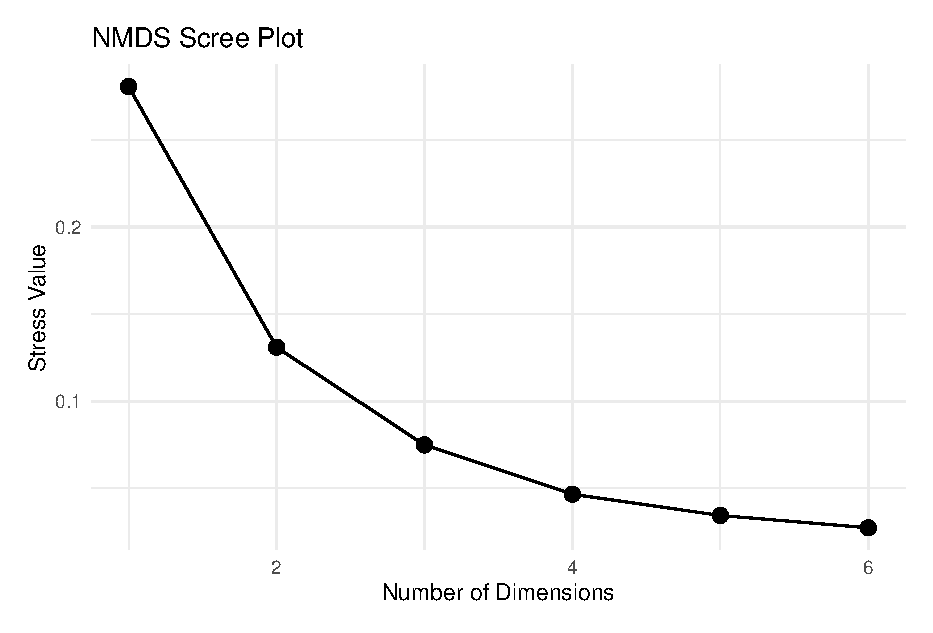
\includegraphics{images/stress_plot.eps}
    \caption{Scree plot for the MDS analysis.}
    \label{fig:stress_plot}
\end{figure}
%--------------------------------------------------------------------------
\section{Results} \label{sec:acousticlandscape:results}
%--------------------------------------------------------------------------
\subsection{Acoustic space of voice quality} \label{sec:acousticlandscape:space}
As mentioned above results of the MDS analysis can be represented in a two-dimensional space, as shown in Figure~\ref{fig:nmds12}. In this and all subsequent plots, breathy voice is represented by black, checked voice with orange, rearticulated voice with green, and modal voice with blue. Overall, we see that breathy voice is located to the left of the plot, checked and rearticulated voice are tending to the right, and modal voice is located in the center along the first dimension. The second dimension shows a modal and nonmodal split with modal voice at the bottom of the plot and nonmodal voice at the top.
\begin{figure}[!h]
    \centering
    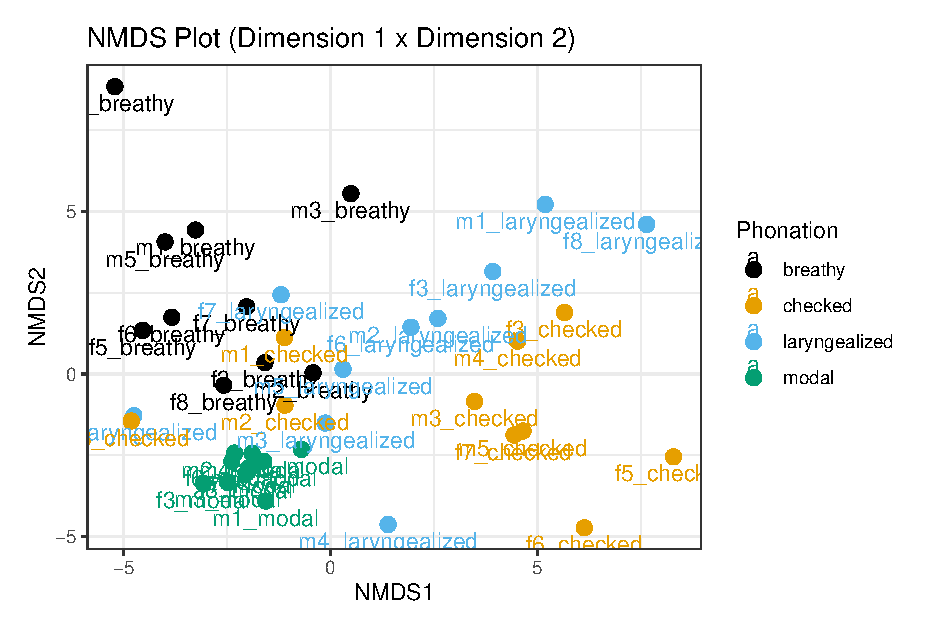
\includegraphics{images/nmds12.eps}
    \caption{Two-dimensional MDS solution showing the first and second dimensions.}
    \label{fig:nmds12}
\end{figure}
    
As mentioned above, the third dimension adds more information about voice quality. The addition of the third dimension helps to spread out the groups along the first dimension, as shown in Figure~\ref{fig:nmds13}. We see that breathy vowels are located at the top of the plot and the two types of creaky voice (checked and rearticulated) are at the bottom of the plot. 

\begin{figure}[!h]
        \centering
        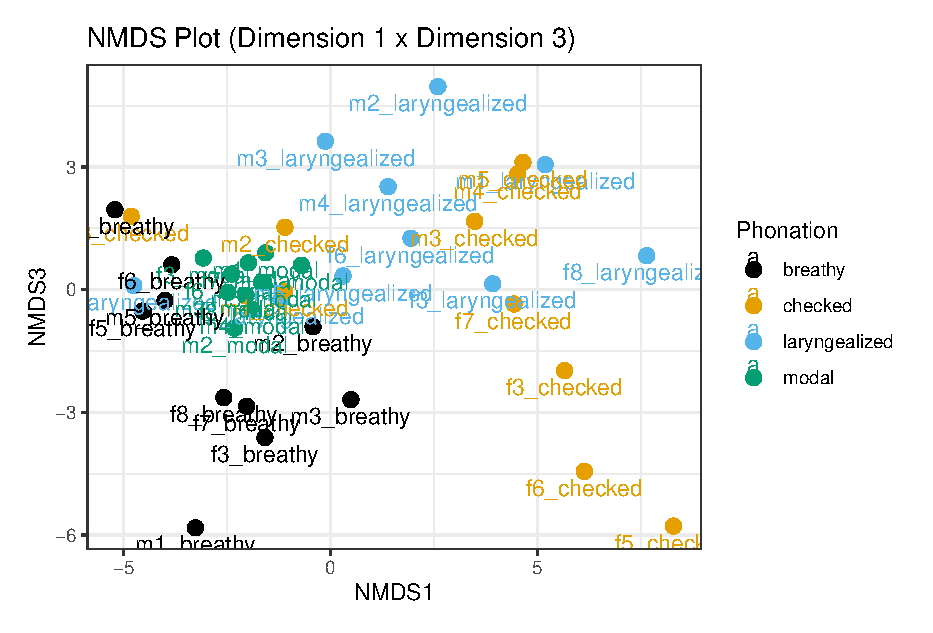
\includegraphics{images/nmds13.eps}
        \caption{Two-dimensional MDS solution showing the first and third dimensions.}
        \label{fig:nmds13}
\end{figure}
    
When the third dimension is added to the second, we see that breathy voices becomes separated from the other nonmodal voice qualities, as shown in Figure~\ref{fig:nmds23}. 

\begin{figure}[!h]
    \centering
    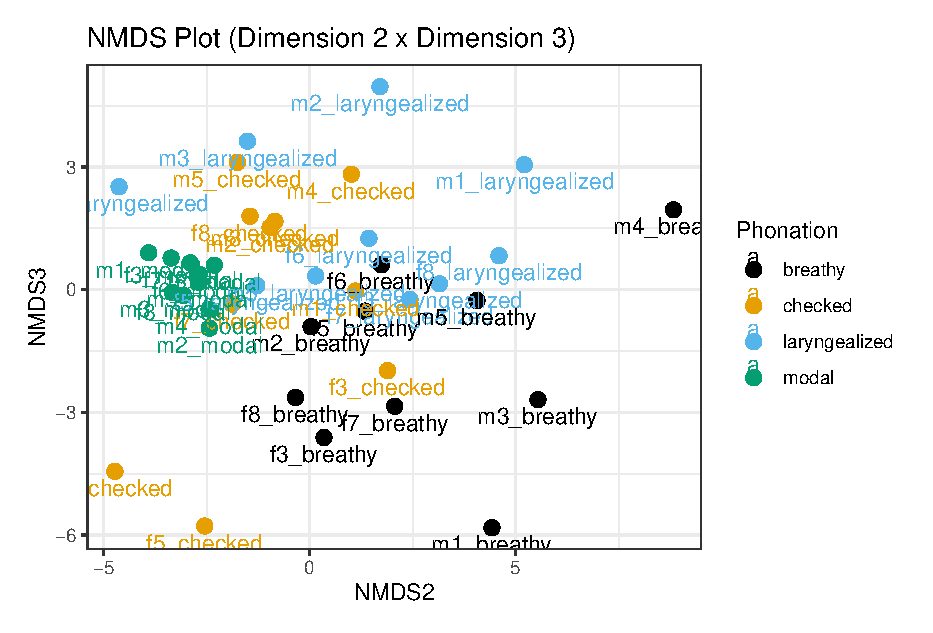
\includegraphics{images/nmds23.eps}
    \caption{Two-dimensional MDS solution showing the second and third dimensions.}
    \label{fig:nmds23}
\end{figure}


\subsection{Acoustic correlates of voice quality} \label{sec:acousticlandscape:correlates}

An additional step to the MDS analysis involves testing which acoustic measures contribute the most weight to the different dimensions. Table~\ref{tab:acoustic_correlates} shows how the 

\begin{table}[ht]
    \centering
    \caption{Weight of each acoustic measure along each dimension of the three-dimensional MDS solution (D1, D2, D3). Parameters that have weights higher than those of other parameters on each dimension are in boldface (weights > 4.0 for D1 and D2, and the weights > 3.0 for D3).} 
    \label{tab:acoustic_correlates}
    \begin{tabular}{lrrr}
    \hline
    Acoustic Measure & D1 & D2 & D3 \\ 
    \hline
    h1h2 & 1.03 & 1.01 & 0.39 \\ 
    h2h4 & 1.15 & 3.98 & 2.13 \\ 
    h1a1 & 2.22 & \textbf{5.15} & 1.84 \\ 
    h1a2 & 2.93 & \textbf{4.66} & 1.00 \\ 
    h1a3 & 2.37 & 3.24 & 0.90 \\ 
    h42k & 1.47 & 0.31 & 1.59 \\ 
    h2kh5k & 3.73 & 0.73 & 0.84 \\ 
    h2 & 1.76 & 0.94 & \textbf{4.09} \\ 
    h4 & 0.79 & 4.28 & 0.10 \\ 
    a1 & \textbf{4.96} & \textbf{5.48} & 0.17 \\ 
    a2 & \textbf{5.30} & \textbf{4.90} & 1.38 \\ 
    a3 & \textbf{4.54} & 2.91 & 1.11 \\ 
    cpp & 4.08 & 0.10 & 1.68 \\ 
    hnr05 & \textbf{5.66} & 1.47 & 1.81 \\ 
    hnr15 & 3.95 & 2.68 & \textbf{3.08} \\ 
    hnr25 & 3.15 & 1.63 & \textbf{3.42} \\ 
    hnr35 & 2.86 & 0.55 & \textbf{3.19} \\ 
    soe & 2.09 & 0.78 & 0.36 \\ 
    shr & 2.39 & 0.50 & 0.47 \\ 
    energy & 2.22 & 3.91 & 0.64 \\ 
    h1\_resid & 1.75 & 0.97 & \textbf{4.24} \\ 
    \hline
    \end{tabular}
\end{table}

%--------------------------------------------------------------------------
\section{Discussion} \label{sec:acousticlandscape:discussion}
%--------------------------------------------------------------------------

\chapter{Trees reveal the importance of measures in SLZ} \label{ch:bagging}

%--------------------------
\section{Introduction} \label{sec:bagging_intro}
%--------------------------

The MDS analysis presented in Chapter~\ref{ch:acousticlandscape} helps us to understand the acoustic landscape of SLZ. This helps reveal the multidimensional nature of voice quality and how all the acoustic measures work together to produce that acoustic landscape. The chapter also discussed how certain measures contributed more weight than other acoustic measures to each of the different dimensions. However, it does not tell us what measures are more important in separating the voice qualities from from one another. This is where decision trees can be most helpful.

%--------------------------
\section{What are Decision Trees} \label{sec:bagging_what}
%--------------------------

Decision trees are a statistical tool that helps to reveal which variables divide the space under investigation. Essentially, this is done by stratifying or segmenting the predictor space into some number of simpler regions. The rules that divide the space into these regions are based on some aspect of the variables (see \cite{hastieElementsStatisticalLearning2009,jamesIntroductionStatisticalLearning2021} for explanations on the statistics and how to perform these analyses in R). 

These trees can be used for both regression and classification. In the case of regressions, it splits the predictor space into regions and calculates how the item under discussion behaves in each region. This process of splitting into regions and calculating how something responds in that region continues until some stopping rule is applied, which is usually defined to some number of terminal nodes. This resulting tree is rather large and is then pruned based on the cost-complexity pruning to a subset of itself. This subsetted tree is the tree that has minimized its cost-complexity criterion of all potential subsets. Meaning that it balances the trade-off between the complexity of the tree and its fit to the data. 

In the case of classification, the algorithms that result in a tree are very similar to those used for regression trees. The main difference in algorithm comes from what is used to split the nodes and how the tree is pruned. Additionally, instead of predicting a continuous outcome like with regression trees, classification trees predict a categorical outcome. The predictor space is divided into regions, and within each region, the majority class is assigned as the predicted class for that region. This process continues until a stopping rule is applied, similar to regression trees. The resulting tree can also be pruned to avoid overfitting, using a cost-complexity criterion.

Decision trees are easy to interpret and visualize, making them an ideal choice for understanding the structure of data and how the different predictors interact with data \citep{hastieElementsStatisticalLearning2009,jamesIntroductionStatisticalLearning2021}.

%-----------------------------
\section{Decision trees in linguistics}\label{sec:bagging_DecisionTrees}
%-----------------------------

The use of decision trees in linguistics is not new. One of the first uses was done by \citet{tagliamonteModelsForestsTrees2012}, where they were illustrated the use of decision trees in investigating which sociolinguistic factors were the most important in the use of \textit{was} versus \textit{were} in York English. Recently, decision trees were used to show which acoustic measures were the most important in making the split in the acoustic space for voice quality \citep{keatingCrosslanguageAcousticSpace2023}. 

In their study, \citet{keatingCrosslanguageAcousticSpace2023} performed a simple decision tree analysis to supplement their MDS analysis of voice quality in 11 languages. The results of this analysis are shown in Figure~\ref{fig:keating_tree}. Decision trees like the one in Figure~\ref{fig:keating_tree}, show the binary splits that are made in the space and what predictor, and the value of that predictor, makes that split. In the case of \citeauthor{keatingCrosslanguageAcousticSpace2023}'s (\citeyear{keatingCrosslanguageAcousticSpace2023}) tree, the first split is made on the harmonics-to-noise ratio over the frequency range from 0 Hz to 500 Hz for the middle third of each vowel. This split is made at the z-score of 0.48. If the value of the predictor is greater or equal to 0.48, the dominate voice quality of that region is modal. If, however, that HNR < 500 Hz value is less than 0.48, the region needs to be further split. 

\begin{figure}[!h]
    \centering
    \includegraphics[width = 0.9\linewidth]{images/keating_tree.pdf}
    \caption{Classification tree of phonation categories from \citet{keatingCrosslanguageAcousticSpace2023}. Abbreviations used in this figure are: {HNR05_means002}: harmonics-to-noise ratio over the frequency range from 0 Hz to 500 Hz for the middle third of each vowel; {SHR_means002}: subharmonic-to-harmonic ratio for the middle third of each vowel; {H1H2c_means002}: H1* − H2* for the middle third of each vowel; B: breathy, M: modal, and C: creaky phonation categories.}
    \label{fig:keating_tree}
\end{figure}

The next split in the region is made on the subharmonic-to-harmonic ratio for the middle third of each vowel. If the value of this predictor is less than 0.0024, the voice quality is classified as breathy. If the value is greater than or equal to 0.0024, the region needs to be split further.

The final split in the region is made on the H1* - H2* for the middle third of each vowel. If the value of this predictor is less than 0.45, the voice quality is classified as creaky. If the value is greater than or equal to 0.45, the voice quality is classified as modal. This tree shows that using only three acoustic measure, one can classify the voice quality of the data. This is a powerful tool for understanding the importance of the different acoustic measures in the acoustic space. 

%--------------------------
\section{What is bagging} \label{sec:bagging_bagging}
%--------------------------

Simple decision trees, however, suffer from two main disadvantages. The first is that decision trees can suffer from high variance. In other words, the tree can be very sensitive to small changes in the data that it was trained on. The second disadvantage is that decision trees do not have the same predictive accuracy as other regression or classification models (see \cite{hastieElementsStatisticalLearning2009} for discussion).

One way to overcome these disadvantages, is to make use of a technique called bootstrap aggregating, or bagging \citep{breimanBaggingPredictors1996}. This means that instead of growing a single tree on the data like in simple decision trees, we grow many trees on random samples of the data until we reach a given number of trees. Once these trees are grown, we then average across the trees to get a more stable prediction of how the regions are split and what predictors are most important in making those splits. This averaging across the trees help to explain the variance in the data and improve the predictive accuracy of the model. However, this comes at the cost of interpretability. 

In decision trees, we usually represent the splits in the data as a tree. When we using bagging, because of the large numbers of trees that are grown, it is impossible to represent the results in this way. Instead of using a tree, we use variable importance measures to understand which predictors are most important in making the splits in the data. There are two measures that are commonly used to understand variable importance in bagging trees: the residual sum of squares (RSS) for regression trees and the Gini index for classification. In regression trees, the amount that the RSS is decreased due to the splits over a given predictor is recorded and averaged across all the trees. In classification trees, the total amount that the Gini index is decreased for each predictor and averaged across all the trees. The higher the value of the RSS or Gini index, the more important that predictor is in making the splits in the data. These are then graphed to show the importance of each predictor in the data with the most important predictors at the top of the graph.

In many instances of bagging trees, the exact number of trees needed to be grown is not known \textit{a priori}. Instead, the number of trees is determined by the user and is usually determined by the number of trees that are needed to stabilize the prediction. This is done by comparing multiple models that where built with different numbers of trees and determining which number of trees produces the most stable prediction. This is done by comparing the predictions of the different models and calculating the variance of the predictions across the different models. The model that produces the most stable prediction is the one that is chosen.

In this chapter, I will use bagging trees to understand the importance of the different acoustic measures in making the splits in the acoustic space of SLZ. This will help to understand which measures are most important in separating the different voice qualities from one another.

%--------------------------
\section{Bagging Trees in SLZ} \label{sec:bagging_slz}
%--------------------------

Using the same data as in Chapter~\ref{ch:acousticlandscape}, I will use bagging trees to understand the importance of the different acoustic measures in making the splits in the acoustic space of SLZ. In order to determine the number of trees that are needed to stabilize the prediction, I compared models with different numbers of trees. The results of this comparison are shown in Figure~\ref{fig:bagging_tree}.

\begin{figure}[!ht]
    \centering
    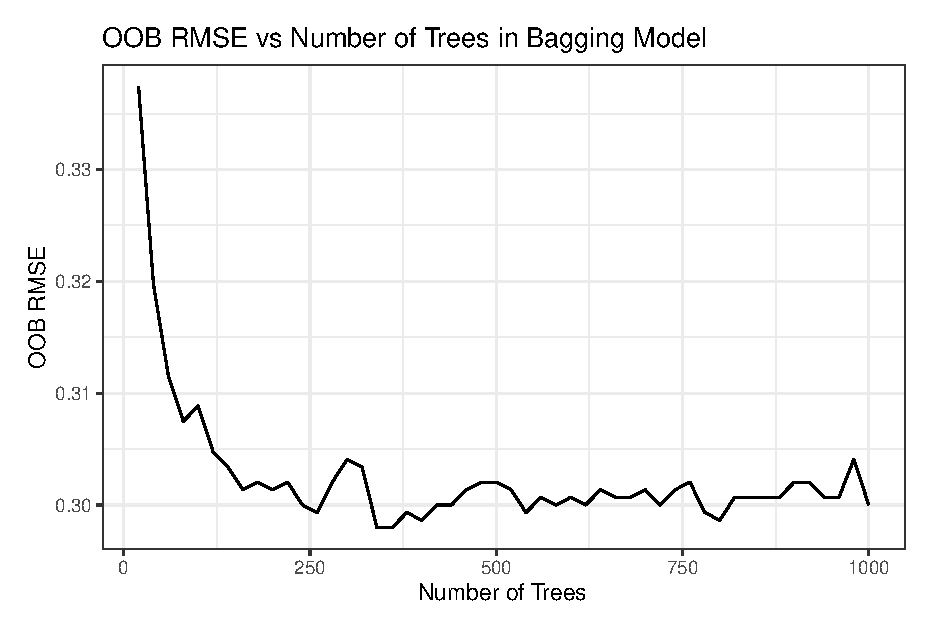
\includegraphics[width = 0.9\linewidth]{images/bagging_numbers.eps}
    \caption{Plot showing the out-of-bag error as a function of the number of trees ran in the bagging models.}
    \label{fig:bagging_tree}
\end{figure}

From Figure~\ref{fig:bagging_tree}, it is clear that the out-of-bag error stabilizes at approximately 400 trees. This means that the number of trees that are required for the the bagging model to be the most stable is also 400 trees. In order to further insure the stability of the model, I also ran a 10-fold cross-validation on the bagging model with 400 trees. The results of this model are shown in Figure~\ref{fig:bagging_importance}.

\begin{figure}[!ht]
    \centering
    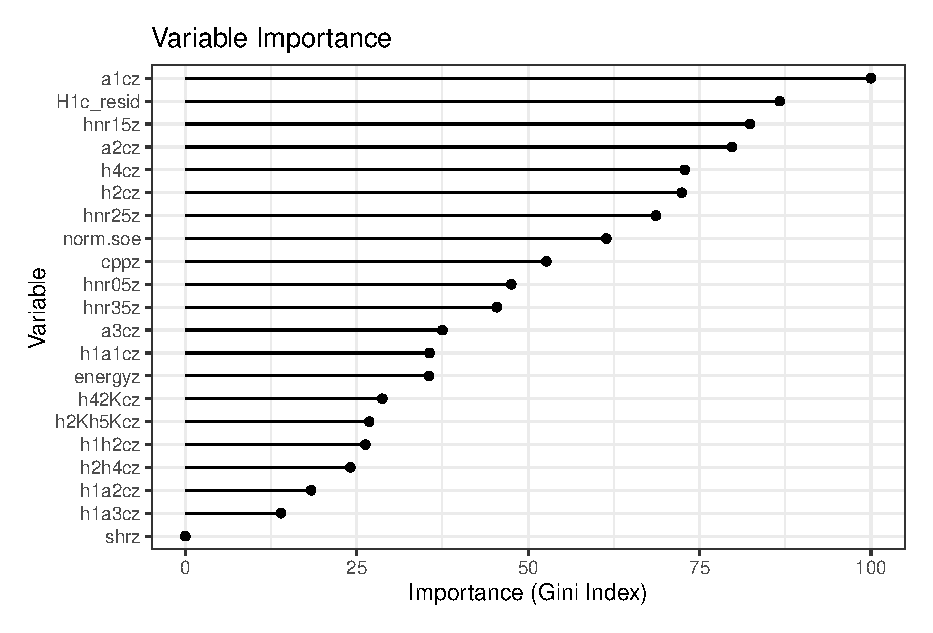
\includegraphics[width = 0.9\linewidth]{images/vip_bagging.eps}
    \caption{Variable importance plot showing the importance of the different acoustic measures in the bagging model based on the total amount that the Gini index is decreased by splits over a given predictor, averaged over all 400 trees.}
    \label{fig:bagging_importance}
\end{figure}

From Figure~\ref{fig:bagging_importance}, the variables with the largest mean decrease in Gini index are A1* (the amplitude of the harmonic closest to the first formant), residual H1*, and the harmonics-to-noise ratio over the frequency range from 0 Hz to 1500 Hz (HNR 1500 Hz). This means that these three variables are the most important in making the splits in the acoustic space of SLZ. This is consistent with the results of the MDS analysis in Chapter~\ref{ch:acousticlandscape}, where these three variables were some of the variables that contributed the most to the different dimensions of the acoustic space. 

%--------------------------
\section{Discussion of the bagging results} \label{sec:bagging_discussion}
%--------------------------

It is interesting to not that in both the MDS analysis and the bagging trees, the same three variables are found to play a role in the acoustic space of SLZ. These two analyses complement each other and help us to better understand what measures to focus are attention on. From Chapter~\ref{ch:acousticlandscape}, we saw that the acoustic measure A1* was heavily weighted for both dimensions 1 and 2. It is not surprising then that this measure would rank so high in the variable importance.

The other two measures that the bagging analysis found to be of most importance are the measures residual H1* and HNR 1500 Hz. These two measures were also important for the analysis in Chapter~\ref{ch:acousticlandscape}. However, they were only heavily weighted for dimension 3. 

The rest of this section will discuss each of the measures that were found to be important in the bagging analysis and how they relate to the different voice qualities in SLZ and other linguistic phenomena. 

%--------------------------
\subsection{Importance of A1*} \label{sec:bagging_a1}
%--------------------------

The measure that was found to be the most important for classifying SLZ's phonation contrasts was A1*. This measure captures the amplitude of the harmonic closest to the first formant. This measure is typically not found in voice quality research except as a way to normalize the amplitude of the first harmonic (i.e., H1*). This goes back to \citet{fischer-jorgensenPhoneticAnalysisBreathy1968} who used this as one of the ways to correct for the high pass filtering, in addition to the widely used H1*$-$H2* measure. However, A1* as a standalone measure is not typically used in voice quality research. Therefore what we are to make of this measure's importance in SLZ is not clear as is its behavior in regards to the different phonations. 

When we look at how A1* is distributed across the different voice qualities in SLZ, as seen as Figure~\ref{fig:a1}, we see that modal vowels are found at the top of the chart with the other phonation contrasts located lower on the chart. The phonation that is found at the bottom of the chart is breathy voice. 
\begin{figure}[!ht]
    \centering
    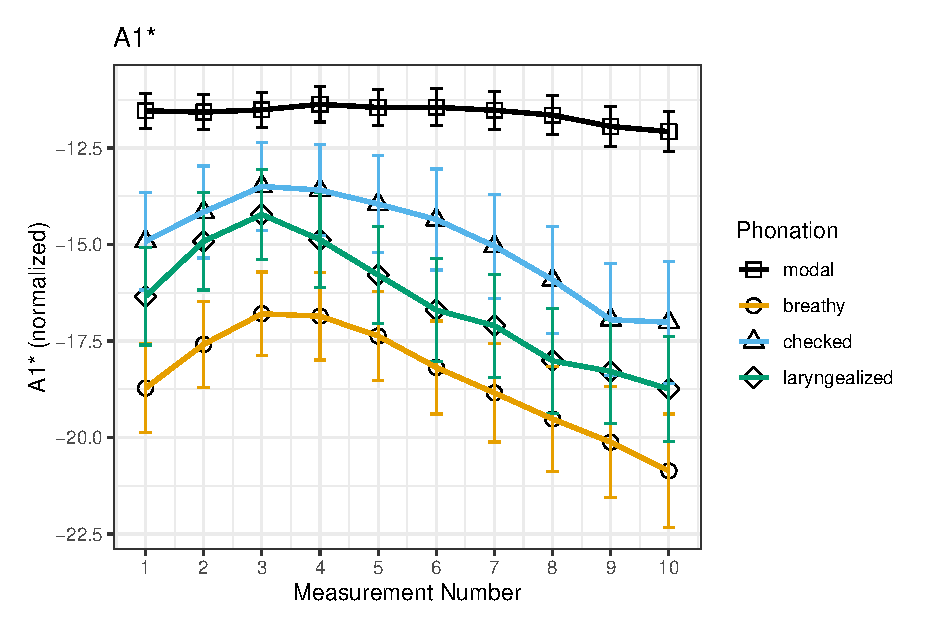
\includegraphics[width = 0.9\linewidth]{images/slz_a1c.eps}
    \caption{Plot showing the distribution of A1* across the different voice qualities in SLZ.}
    \label{fig:a1}
\end{figure}

This pattern of behavior, especially for breathy versus modal, is very similar to what is found in other languages and descriptions of the behavior of the first formant in breathy voice contexts. For example differences in the first formant are typically used to distinguish register differences in Southeast Asian languages \citep{brunelleRegisterEasternCham2005,brunelleDialectExperiencePerceptual2012,brunelleTonePhonationSoutheast2016}.

As described in \citet{brunelleTonePhonationSoutheast2016}, many of the languages of Southeast Asia have what is called register. The linguistic term register is defined as ``the redundant use of pitch, voice quality, vowel quality, and durational differences to distinguish (typically two) contrastive categories'' \citep[193]{brunelleTonePhonationSoutheast2016}, and was first used by \citet{hendersonMainFeaturesCambodian1952} to describe the categorical contrasts found in Khmer. The characteristics that define the higher and lower registers are found in Table~\ref{tab:register_correlates}.

\begin{table}[!ht]
    \centering
    \caption{Possible phonetic correlates of register. From \citet{brunelleTonePhonationSoutheast2016}.}
    \label{tab:register_correlates}
    \begin{tabular}{ll}
        \lsptoprule
        \textbf{Higher Register} & \textbf{Lower Register} \\
        \hline
        Higher pitch & Lower pitch \\
        Tense/Modal voice & Lax/Breathy voice \\
        Monophthongs/shorter vowels & Diphthongs/longer vowels \\
        Raised F1/lower vowels/[+ATR] & Lowered F1/higher vowels/[-ATR] \\
        Plain stops/shorter VOT & Aspirated stops/longer VOT \\
        \lspbottomrule
    \end{tabular}
\end{table}

From this table, the lower register is what interests us here. The lower register is associated with breathy voice and a lowered first formant. This is very similar to what we see in Figure~\ref{fig:a1} where breathy voice is associated with a lower A1* than modal voice. It is not entirely clear if the amplitude of the first formant also behaves in this same way in these languages as the the lowering of the first formant's frequency. 

There is evidence that breathy voice frequently has a lower first formant than modal voice in paralinguistic settings for English \citep{lottoEffectVoiceQuality1997}.  However, these studies do not discuss the amplitude of the first formant but rather the frequency of the first formant.

Another comparison can be found in nasality research, where this measure is discussed quite extensively either alone or in association with the nasal pole (e.g., \cite{chenAcousticCorrelatesEnglish1997,delvauxPerceptionContrasteNasalite2009,macmillanIntegralityNasalizationF11999,pruthiAcousticParametersAutomatic2004,,schwartzAcousticsNormalNasal1968,stevensAcousticPhonetics2000,stylerAcousticalPerceptualFeatures2015,stylerAcousticalFeaturesVowel2017}). These studies discuss how in nasalized contexts the amplitude of the first formant is typically found to be lower than in oral ones, again similar to what we see in Figure~\ref{fig:a1}.

There is a large body of research that discusses that nasality is closely associated with breathy voice or the glottal consonants, in a phenomenon called \textit{rhinoglottophilia} \citep{matisoffRhinoglottophiliaMysteriousConnection1975,ohalaPhoneticExplanationsNasal1975,ohalaPhoneticsNasalPhonology1993,bennettMayanPhonology2016}. In \citet{blevinsEvolutionPonapeicNasal1993,matisoffRhinoglottophiliaMysteriousConnection1975}, this association is attributed to the acoustic and perceptual similarities between nasalization and breathy voice. In one study, \citet{garellekBreathyVoiceNasality2016} showed that in nasalization in three different Yi languages were associated with breathy voice. Leading the authors to suggest that breathy voice during nasalization can arise from misperception or as a type of phonetic enhancement. 

In regards to what is going on in SLZ, it is not clear if the lowering of A1* for breathy voice can be attributed to the same observations as discussed above. I suggest that there are three different possibilities to explain what is going on in SLZ. Because SLZ does not have phonemic nasaliZation, it is possible that speakers of SLZ are using nasalization as a way to phonetically enhance the the contrast of breathy voice. Essentially, the reverse of what was reported by \citet{garellekBreathyVoiceNasality2016}. This possibility could be tested acoustically by performing an experiment to detect nasal airflow during breathy vowels. The second possibility is that the same measures that work for detecting nasality can also be used to detect breathy voice. This second possibility could be easily tested by examining whether A1* and the other measures for nasality work in other breathy voice contexts cross-linguistically. The third possibility is that the lowering of A1* is a result of sub-glottal resonances which is much harder to test than the other two possibilities. 

%--------------------------
\subsection{Importance of Residual H1*} \label{sec:bagging_residual}
%--------------------------
As residual H1* is a type of spectral slope measure it is expected to show similar behavior to other spectral slope measures. Namely, breathy voice should be associated with a higher score than modal voice. Since the two types of laryngealization are closely associated with creaky voice, they should be associated with a lower score than modal voice. Additionally, there is a temporal difference between the two types of laryngealization, it is expected that checked voice will have a lower score toward the end of the vowel and  rearticulated voice will have a lower score in the middle of the vowel. 

In Figure~\ref{fig:residualH1}, we see that are predictions are correct. Breathy voice is associated with a higher score than modal voice. The two types of laryngealization are associated with a lower score than modal voice.

\begin{figure}[!ht]
    \centering
    \includegraphics[width = 0.9\linewidth]{images/slz_residual_h1c.eps}
    \caption{Plot showing the distribution of residual H1* across the different voice qualities in SLZ.}
    \label{fig:residualH1}
\end{figure}

A further analysis of the results of this measure using generalized additive (mixed) models (GAM(M)s; \cite{hastieGeneralizedAdditiveModels1986,woodGeneralizedAdditiveModels2017,soskuthyGeneralisedAdditiveMixed2017,wielingAnalyzingDynamicPhonetic2018}) shows that the temporal behavior of the two types of laryngealization is also correct. Checked voice is associated with a lower score toward the end of the vowel and rearticulated voice is associated with a lower score in the middle of the vowel. Additionally, the results of the GAMM show that for the first three time points there is no significant difference between breathy and modal voice. Suggesting that breathy voice is more closely associated with the latter part of the vowel than the beginning. The full results of the GAMM for residual H1* are discussed in Chapter~\ref{ch:residual_h1}.

%--------------------------
\subsection{Importance of the HNR \textless 1500 Hz} \label{sec:bagging_hnr}
%--------------------------

The acoustic measure HNR $<$ 1500 Hz is a harmonics-to-noise ratio measure that is calculated over the frequency range from 0 Hz to 1500 Hz and is a measure of the amount of noise in the signal or in other words it is measure of periodicity. In these measures, modal voice is associated with a higher score than non-modal phonations. This is because modal voice is associated with a higher degree of periodicity than non-modal phonations as a-periodicity is a defining feature of non-modal phonations (e.g., \cite{hillenbrandAcousticCorrelatesBreathy1996,blankenshipTimeCourseBreathiness1997,kentVoiceQualityMeasurement1999}).

As seen in Figure~\ref{fig:hnr1500}, this is exactly what we see in SLZ. Modal voice is associated with a higher score than non-modal phonations. Among the non-modal phonations, breathy and rearticulated voice have a higher HNR $<$ 1500 Hz than checked voice. 

\begin{figure}[!ht]
    \centering
    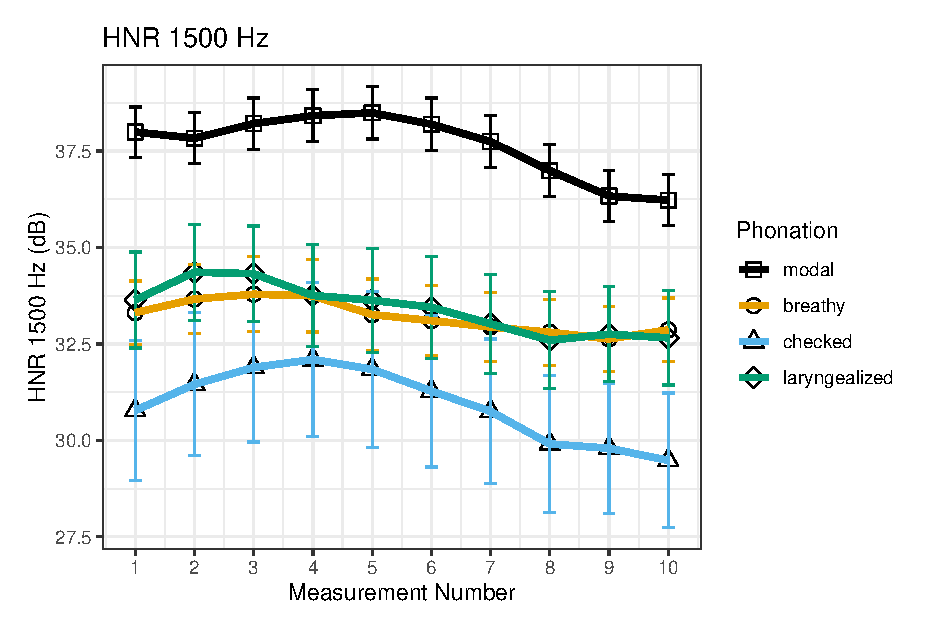
\includegraphics[width = 0.9\linewidth]{images/slz_hnr15.eps}
    \caption{Plot showing the distribution of HNR $<$ 1500 Hz across the different voice qualities in SLZ.}
    \label{fig:hnr1500}
\end{figure}

The fact that breathy and rearticulated voice have a higher HNR $<$ 1500 Hz than checked voice is not surprising. As discussed in Chapter~\ref{ch:SLZ}, breathy and rearticulated voices are associated with more modal-like qualities than checked voice. In most instances of rearticulated voice, the vowel is produced with modal voice except for a small portion of the middle of the vowel where the vowel is produced with creaky voice or a glottal occlusion. Breathy voice typically appears  very periodic but with a high degree of noise in the signal. Checked voice on the other hand is typically the shortest of the non-modal phonations and is associated with a high degree of aperiodicity in the signal from the creaky voice that is produced at the end of the vowel. This is why checked voice has the lowest HNR $<$ 1500 Hz of the non-modal phonations.

This measure will be very important in Chapter~\ref{ch:testing_lc}, where this measure will be used to test the predictions of the laryngeal complexity hypothesis.

%--------------------------
\section{Conclusion} \label{sec:bagging_conclusion}
%--------------------------

In conclusion, the results of the bagging analysis show that the acoustic measures A1*, residual H1*, and HNR $<$ 1500 Hz are the most important in making the splits in the acoustic space of SLZ. These three measures are also the measures that were found to be the important in the MDS analysis in Chapter~\ref{ch:acousticlandscape}. This suggests that these three measures play an important role in defining and characterizing the different voice qualities from one another in SLZ. 


%--------------------------------------------------------------------------
\chapter{Testing the laryngeal complexity in SLZ} \label{ch:testing_lc}
%--------------------------------------------------------------------------

%--------------------------------------------------------------------------
\section{What is Laryngeal Complexity?}\label{sec:what_is_lc}
%--------------------------------------------------------------------------

Laryngeal complexity is defined as the contrastive use of tone and phonation on the same syllablic nucleus \citep{silvermanLaryngealComplexityOtomanguean1997,silvermanPhasingRecoverability1997}. This use of both tone and phonation on the same nucleus is one of the defining characteristics of the Oto-Manguean languages \citep{silvermanLaryngealComplexityOtomanguean1997}. However, it is not limited to just these languages. It has also been used to describe the behavior of tone or pitch in languages outside of the Oto-Manguean languages; such as the Tibeto-Burman languages of Mpi and Tamang \citep{silvermanLaryngealComplexityOtomanguean1997,silvermanPhasingRecoverability1997} and the Mayan language Yucatec Mayan \citep{frazierPhoneticsYucatecMaya2013}. 
%, and the Germanic language Danish \citep{frazierPhoneticsYucatecMaya2013,penaStodTimingDomain2022,penaProductionPerceptionStod2024}.


%--------------------------------------------------------------------------
\subsection{Phasing and recoverability}\label{sec:phasing_and_recoverability}
%--------------------------------------------------------------------------

According to \citet{silvermanLaryngealComplexityOtomanguean1997,silvermanPhasingRecoverability1997}, one of the defining aspects of laryngeal complexity is the concept of phasing and recoverability. Under this idea, in laryngeally complex vowels the phonation and tone are phased with respect to one another in way that lends itself to a listener's ability to recover the underlying phonation and tone. In practical terms this means that laryngeally complex vowels are composed of two components: a modal voice portion of the vowel where tone is realized, and a non-modal voice portion of the vowel where phonation is realized. For the researcher that means that there are two distinct portions of the vowel that can be analyzed separately and that need to be analyzed temporally rather than spectrally \citep[237]{silvermanLaryngealComplexityOtomanguean1997}.

For example, in the Oto-Manguean language Jalapa Mazatec, breathiness or creakiness is realized only on the first portion of the vowel either as full laryngeal consonant or as a laryngeal feature on the vowel \citep[238]{silvermanLaryngealComplexityOtomanguean1997}. The second portion of the vowel is realized as a modal voice vowel with one of the three tones belonging to the tonemes of the language. This means that the breathiness or creakiness is phased with respect to the tone.

\citeauthor{silvermanLaryngealComplexityOtomanguean1997} argues that there are three principles that help explain why laryngeal complexity needs to be temporally ordered or phased: (i) sufficient acoustic distance, (ii) sufficient articulatory compatibility, and (iii) optimal auditory salience. 

%--------------------------------------------------------------------------
\subsubsection{Sufficient acoustic distance}\label{sec:sufficient_acoustic_distance}
%--------------------------------------------------------------------------

\citet{silvermanLaryngealComplexityOtomanguean1997} argues that sufficient acoustic distance is necessary for the recoverability of the phonation and tone. As Silverman explain, listeners do not rely on the fundamental frequency alone to perceive pitch. Instead, listeners use the harmonic spacing and the pulse period in the signal to perceive pitch \citep{ritsmaFrequenciesDominantPerception1967,remezIntonationSinusoidalSentences1993}. For modal phonation, this means that the harmonic spacing and pulse periods are present and encode a salient pitch value. However, during non-modal phonation, the harmonic spacing and pulse periods are often obscured or not present.

For breathy voice, this means that there is a general weakening 
of the harmonic structure which makes it difficult to recover the pitch by the listener \citep{silvermanPhasingRecoverability1997}. Creaky voice on the other had obscures the pulse periods due to its aperiodic and unstable glottal vibration \citep{ladefogedSoundsWorldLanguages1996}. This is what was observed in Mazatec where the harmonic structure is gone and the pulses are indiscernible \citep{kirkQuantifyingAcousticProperties1993}. Additionally, the perception of pitch is rendered indiscernible when the pulse periods are varied by 10\% or more \citep{rosenbergPitchDiscriminationJittered1966}.

These observations lead \citet{silvermanLaryngealComplexityOtomanguean1997} to conclude that if a period glottal wave is either obscured (as with breathy voice) or not present (as with creaky voice), the acoustic signal cannot encode a salient pitch value. This means that the phonation and tone must be phased with respect to one another in order for the listener to recover the underlying phonation and tone. I will return to this point in Section~\ref{sec:discussion_of_lc}.

%--------------------------------------------------------------------------
\subsubsection{Sufficient articulatory compatibility}\label{sec:sufficient_articulatory_compatibility}
%--------------------------------------------------------------------------

Another important point for the \citeauthor{silvermanLaryngealComplexityOtomanguean1997}'s theory about laryngeal complexity has to deal with the articulatory compatibility of the phonation and tone. One of the guiding ideas behind this principle is that there is a principle of least effort in biological motor systems such as with speech production \citep{lindblomEconomySpeechGestures1983}. According to \citet{lindblomEconomySpeechGestures1983}, speech gestures can be thought of as distinct motor goals in our speech production system. These goals are achieved by the speaker through the coordination of the articulators with the least amount of effort. This means that that the gestures are coordinated in such a way that they are compatible with one another. This manifests itself either through sequencing or coarticulation of the gestures.

A good example of this comes from nasalization. In nasal contexts, the velum is lowered to allow air to pass through the nasal cavity, creating a nasal sound. This velum lowering gesture is compatible with the gestures needed in the oral cavity to produce different vowel qualities. This is what leads to the production of nasal vowels in languages like French or Portuguese. Additionally, this lowering also occurs in languages that do not have contrastive nasal vowels, such as English, where the velum is lowered in anticipation of a nasal consonant. This lowering of the velum is compatible with the gestures needed to produce the vowels in the oral cavity \citep[e.g.,][]{ohalaPhoneticExplanationsNasal1975,chenAcousticCorrelatesEnglish1997,stylerAcousticalPerceptualFeatures2015}.

According to \citeauthor{silvermanLaryngealComplexityOtomanguean1997}'s theory of laryngeal complexity, this idea of articulatory compatibility is also driving the need to phase phonation and tone. In the case of laryngeal complexity this is because it is assumed that both tone and phonation are produced by the larynx, more specifically the vocal folds and the glottis. This comes from early work on phonation and tone. For tone, \citet{ohalaProductionTone11978} showed that pitch was controlled primarily by the tensing or laxing of the vocal folds which changed the rate at which the vocal folds vibrate. For phonation, it was similarly shown that the amount the vocal folds where held open or closed determined the type of phonation that was produced \citep{ladefogedSoundsWorldLanguages1996}. This aspect of phonation was shown in Figure~\ref{fig:phonation_types} and repeated here as Figure~\ref{fig:phonation_types_repeat}. 

\begin{figure}[h!]
    \centering
    \begin{tikzpicture}
        % Draw the line with arrows at both ends
        \draw[<->, line width=0.5mm] (0,0) -- (10,0);
        
        % Labels underneath the line
        \node[below] at (0,0) {[h]};
        \node[below] at (2,0) {Breathy};
        \node[below] at (5,0) {Modal};
        \node[below] at (8,0) {Creaky};
        \node[below] at (10,0) {[ʔ]};
        
        % Labels above the line
        \node[above] at (0,0) {Open Glottis};
        \node[above] at (10,0) {Closed Glottis};
    \end{tikzpicture}
    \caption{A diagram showing the relationship between breathy, modal, and creaky phonation types. Based on \citet{gordonPhonationTypesCrosslinguistic2001}.}
    \label{fig:phonation_types_repeat}
\end{figure}

For \citeauthor{silvermanLaryngealComplexityOtomanguean1997}'s \citeyear{silvermanLaryngealComplexityOtomanguean1997} theory of laryngeal complexity, the articulatory mechanisms for tone and phonation are exactly the same which leads to a need to phase the two in order to optimally make use of the same articulatory gestures. However, there is a growing body of literature that shows that tone and phonation is much more complex and is reliant on the entire larynx not just the vocal folds (e.g., \cite{eslingVoiceQualityLaryngeal2019}). This matter will be picked up again in Section~\ref{sec:discussion_of_lc} and Chapter~\ref{ch:modeling_lc}.

%--------------------------------------------------------------------------
\subsubsection{Optimal auditory salience}\label{sec:optimal_auditory_salience}
%--------------------------------------------------------------------------


%--------------------------------------------------------------------------
\subsection{Implicational hierarchy of laryngealization}\label{sec:implicational_hierarchy}
%--------------------------------------------------------------------------

Another aspect of \citeauthor{silvermanLaryngealComplexityOtomanguean1997}'s \citeyear{silvermanLaryngealComplexityOtomanguean1997} laryngeal complexity theory is that there is an implicational hierarchy in the phasing and ordering of phonation and tone. This hierarchy is based on how laryngealization appears in three Oto-Manguean languages. In this implicational hierarchy laryngealization can only appear in three ways: prevocalic, postvocalic, or interrupted. In the prevocalic case, the laryngealization appears before the vowel. In the postvocalic case, the laryngealization appears after the vowel. In the interrupted case, the laryngealization interrupts a vowel and appears in the middle.

According to \citet{silvermanLaryngealComplexityOtomanguean1997}, if a language has interrupted laryngealization, it must also have postvocalic laryngealization. If a language has postvocalic laryngealization, it must also have prevocalic laryngealization. In support of his claims \citet{silvermanLaryngealComplexityOtomanguean1997} provides data from three Oto-Manguean languages: Jalapa Mazatec, Comaltepec Chinantec, and Copala Trique. These languages are shown in Table~\ref{tab:implicational_hierarchy}.

\begin{table}[!ht]
    \centering
    \caption{Implicational hierarchy of laryngeal complexity. The symbols h and ʔ represent laryngealization. The symbol V represents where the modal vowel is located in relation to the laryngealization.  Modified from \citet{silvermanLaryngealComplexityOtomanguean1997}.} 
    \label{tab:implicational_hierarchy}
    \begin{tabular}{lccc}
        \lsptoprule
        \textbf{Language} & \textbf{Prevocalic} & \textbf{Postvocalic} & \textbf{Interrupted} \\
        \hline 
        Jalapa Mazatec & hV˥, ʔV˥ & $-$ & $-$ \\
        Comaltepec Chinantec & hV˥, ʔV˥ & Vh˥, Vʔ˥ & $-$ \\
        Copala Trique & hV˥, ʔV˥ & Vh˥, Vʔ˥ & VhV˥, VʔV˥ \\
        \lspbottomrule
    \end{tabular}
\end{table}

However, as mentioned by \citet{frazierPhoneticsYucatecMaya2013}, it is not clear how accurate or robust this implicational hierarchy is. The reason for this is because it is not always clear if something is a laryngeal consonant or a laryngeal feature on the vowel. Indeed, \citet{silvermanLaryngealComplexityOtomanguean1997,silvermanPhasingRecoverability1997} treats laryngeal consonants and laryngeal features on vowels as the same thing. For example, in many of the Trique languages, the laryngealization is realized as a laryngeal consonant \citep{dicanioPhoneticsPhonologySan2008,dicanioItunyosoTrique2010,dicanioCoarticulationToneGlottal2012,dicanioPhoneticsFortisLenis2012,dicanioCueWeightPerception2014,dicanioGlottalTogglingItunyoso2020,elliottChicahuaxtlaTriqui2016,hollenbachPhonologyMorphologyTone1984}, but in Jalapa Mazatec, the laryngealization is realized as a laryngeal feature on the vowel \citep{kirkQuantifyingAcousticProperties1993,garellekAcousticConsequencesPhonation2011}. 

Another issue with the implicational hierarchy is that it is based on only three languages. This is a rather small sample size and doesn't capture the full range of variation in the Oto-Manguean languages. For example, in many Mixtec languages, laryngealization is understood to be a feature of the vowel rather than a consonant \citep[e.g.,][]{cortesSanSebastianMonte2023,eischensTonePhonationPhonologyPhonetics2022,gerfenPhonologyPhoneticsCoatzospan1999,gerfenProductionPerceptionLaryngealized2005}. Additionally, in many of this languages, the larngealization can appear either in the middle of the vowel, what \citet{silvermanLaryngealComplexityOtomanguean1997} calls interrupted, or at the end of the vowel \citep[e.g.,][]{cortesSanSebastianMonte2023,eischensTonePhonationPhonologyPhonetics2022}. This is directly in contrast to the implicational hierarchy which states that if a language has interrupted laryngealization, it must also have postvocalic laryngealization and prevocalic laryngealization.

Not only is the violation of the implicational hierarchy the case in Mixtecan languages, it is also the case in other branches of the Oto-Manguean languages. It is often the case that Zapotec languages only have interrupted and postvocalic vowels or just interrupted vowels (see \cite{ariza-garciaPhonationTypesTones2018} for a typology of phonation in Zapotec languages).  

For example, \citet{avelinobecerraTopicsYalalagZapotec2004,avelinoAcousticElectroglottographicAnalyses2010} argues that Yalálag Zapotec only has interrupted laryngealization as a vowel feature and postvocalic laryngealization with a laryngeal consonant. 
    
%--------------------------------------------------------------------------
\section{Previous analyses of laryngeal complexity}\label{sec:previous_analyses}
%--------------------------------------------------------------------------

%--------------------------------------------------------------------------
\subsection{Jalapa Mazatec analysis}\label{sec:jalapa_mazatec_analysis}
%--------------------------------------------------------------------------




%--------------------------------------------------------------------------
\section{Analysis of laryngeal complexity}\label{sec:analysis_of_lc}
%--------------------------------------------------------------------------


%--------------------------------------------------------------------------
\section{Results}\label{sec:results_of_lc}
%--------------------------------------------------------------------------


%--------------------------------------------------------------------------
\section{Discussion}\label{sec:discussion_of_lc}
%--------------------------------------------------------------------------

\citet{humbertConsonantTypesVowel1978} 


%--------------------------------------------------------------------------
\section{Conclusion}\label{sec:conclusion_of_lc}
%--------------------------------------------------------------------------

%--------------------------------------------------------------------------
% Modeling laryngeal complexity
\chapter{Modeling laryngeal complexity} \label{ch:modeling_lc}
%--------------------------------------------------------------------------

%--------------------------------------------------------------------------
\section{The Laryngeal Articulator Model}\label{sec:lam}
%--------------------------------------------------------------------------

\citet{eslingThereAreNo2005,eslingVoiceQualityLaryngeal2019,moisikPhonologicalPotentialsLower2021,moisikMultimodalImagingGlottal2015,moisikModelingBiomechanicalInfluence2014}

\begin{figure}
    \centering
    \begin{tikzpicture}
        \node[draw,circle,minimum size=1cm,inner sep=0pt] (tra) at (0,0) {tra};
        \node[draw,circle,minimum size=1cm,inner sep=0pt] (tfr) at (-2,-1.5) {tfr};
        \node[draw,circle,minimum size=1cm,inner sep=0pt] (tre) at (2,-1.5) {tre};
        \node[draw,circle,minimum size=1cm,inner sep=0pt] (tdb) at (0,-3) {tdb};

        \node[draw,circle,minimum size=1cm,inner sep=0pt] (epc) at (0,-6) {epc};
        \node[draw,circle,minimum size=1cm,inner sep=0pt] (vfo) at (-2,-7.5) {vfo};
        \node[draw,circle,minimum size=1cm,inner sep=0pt] (vfc) at (2,-7.5) {vfc};
        \node[draw,circle,minimum size=1cm,inner sep=0pt] (epv) at (0,-9) {epv};

        \node[draw,circle,minimum size=1cm,inner sep=0pt] (lower_lx) at (-3.5,-6) {↓lx};
        \node[draw,circle,minimum size=1cm,inner sep=0pt] (raised_lx) at (3.5,-6) {↑lx};

        \node[draw,circle,minimum size=1cm,inner sep=0pt] (Lf0) at (-2,-10.5) {Lf0};
        \node[draw,circle,minimum size=1cm,inner sep=0pt] (Hf0) at (2,-10.5) {Hf0};
        
        % Anti-syngeristic
        \draw[<->, dotted, line width=.5mm] (tra.west) to[out=180,in=90] (tfr.north);
        \draw[<->,dotted, line width=.5mm] (tra.east) to[out=0,in=90] (tre.north);
        \draw[<->,dotted, line width=.5mm] (tfr.east) to (tre.west);
        \draw[<->,dotted, line width=.5mm] (tra.south) to (tdb.north);
        \draw[<->,dotted, line width=.5mm] (tfr.south) to[in=180, out=-90] (epc.west);
        \draw[<->,dotted, line width=.5mm] (lower_lx.north) to[in=140,out=40] (raised_lx.north);
        \draw[<->,dotted, line width=.5mm] (lower_lx.east) to (epc.west);
        \draw[<->,dotted, line width=.5mm] (epc.west) to[in=90,out=180] (vfo.north);
        \draw[<->,dotted, line width=.5mm] (vfo.east) to[in=180,out=0] (vfc.west);
        \draw[<->,dotted, line width=.5mm] (vfc.south) to[in=0,out=-90] (epv.east);
        \draw[<->,dotted, line width=.5mm] (epc.south) to[out=-90, in=90] (Hf0.north);
        \draw[<->,dotted, line width=.5mm] (Hf0.south) to[out=-140, in=-40] (Lf0.south);
        \draw[<->,dotted, line width=.5mm] (epv.south) to[out=-90, in=180] (Hf0.west);

        % Syngeristic
        \draw[<->, line width=.5mm] (tdb.west) to[out=180, in=-90] (tfr.south);
        \draw[<->, line width=.5mm] (tdb.east) to[out=0, in=-90] (tre.south);
        \draw[<->, line width=.5mm] (epc.north) to (tdb.south);
        \draw[<->, line width=.5mm] (epc.south) to (epv.north);
        \draw[<->, line width=.5mm] (epc.east) to[in=-90, out=0] (tre.south);
        \draw[<->, line width=.5mm] (lower_lx.north) to[in=-135, out=90] (tfr.west);
        \draw[<->, line width=.5mm] (raised_lx.north) to[in=-45, out=90] (tre.east);
        \draw[<->, line width=.5mm] (Lf0.west) to[in=-90, out =135] (lower_lx.south);
        \draw[<->, line width=.5mm] (raised_lx.west) to (epc.east);
        \draw[<->, line width=.5mm] (Hf0.east) to[in=-90, out=45] (raised_lx.south);
        \draw[<->, line width=.5mm] (epv.south) to[out=-90, in=0] (Lf0.east);
        \draw[<->, line width=.5mm] (epc.east) to[out=0, in=90] (vfc.north);
        \draw[<->, line width=.5mm] (vfo.south) to[out=-90, in=180] (epv.west);
        \draw[<->, line width=.5mm] (vfc.south) to (Hf0.north);
        \draw[<->, line width=.5mm] (vfo.south) to (Lf0.north);
        \draw[<->, line width=.5mm] (epc.south) to[out=-90,in=90] (Lf0.north);
        \draw[<->, line width=.5mm] (lower_lx.south) to[out=-90,in=180] (vfo.west);
        \draw[<->, line width=.5mm] (raised_lx.south) to[out=-90,in=0] (vfc.east);

        % Curly bracket with text
        \draw[decorate,decoration={brace,amplitude=10pt,raise=5pt},thick] (4,0) -- (4,-4) node[midway,xshift=15pt,right=5pt] {\parbox{2cm}{vowel\\quality}};
        \draw[decorate,decoration={brace,amplitude=10pt,raise=5pt},thick] (4,-4) -- (4,-9.5) node[midway,xshift=15pt,right=5pt] {\parbox{2cm}{phonatory\\quality}};
        \draw[decorate,decoration={brace,amplitude=10pt,raise=5pt},thick] (4,-9.5) -- (4,-11) node[midway,xshift=15pt,right=5pt] {\parbox{2cm}{tonal\\quality}};
        \draw[decorate,decoration={brace,amplitude=10pt,raise=5pt},thick] (7,-2) -- (7,-11) node[midway,xshift=15pt,right=5pt] {\parbox{2cm}{voice\\quality}};

        
    \end{tikzpicture}
    \caption{The Laryngeal Articulator Model from \citet{eslingVoiceQualityLaryngeal2019}. This model shows the interactions between the laryngeal articulators (labeled circles). Syngeristic interactions are shown with solid lines, while anti-syngeristic interactions are shown with dotted lines.}
    \label{fig:tra}
\end{figure}
\include{contents/6.conclusion}

%--------------------------------------------------------------------------
%  Bibliography
%--------------------------------------------------------------------------
%------------------------------------
% BIBLIOGRAPHY
%------------------------------------

%\singlespacing
% \nocite{*}
\printbibliography[heading=bibintoc]

\appendix
%Appendix chapter
\chapter{Some Ancillary Stuff}

Ancillary material should be put in appendices, which appear after the
bibliography. 


\end{document}
